\documentclass[conference, onecolumn]{IEEEtran}
\IEEEoverridecommandlockouts
% The preceding line is only needed to identify funding in the first footnote. If that is unneeded, please comment it out.
\usepackage{cite}
\usepackage{amsmath,amssymb,amsfonts}
\usepackage{algorithmic}
\usepackage{graphicx}
\usepackage{textcomp}
\usepackage{xcolor}
\usepackage{subcaption}
\def\BibTeX{{\rm B\kern-.05em{\sc i\kern-.025em b}\kern-.08em
    T\kern-.1667em\lower.7ex\hbox{E}\kern-.125emX}}
\begin{document}

\title{Enhanced Weather Prediction using Machine Learning\\}

\author{
    \IEEEauthorblockN{S.Kayalvili\IEEEauthorrefmark{1}}
    \IEEEauthorblockA{\textit{Department of Artificial Intelligence} \\
    \textit{Kongu Engineering College}\\
    Erode, India \\
    kayalvili.ai@kongu.edu}
    \and
    \IEEEauthorblockN{Gowtham.S\IEEEauthorrefmark{2}}
    \IEEEauthorblockA{\textit{Department of Artificial Intelligence} \\
    \textit{Kongu Engineering College}\\
    Erode, India \\
    gowthams.22aim@kongu.edu}
    \and
    \IEEEauthorblockN{Jay Akash.V\IEEEauthorrefmark{3}}
    \IEEEauthorblockA{\textit{Department of Artificial Intelligence} \\
    \textit{Kongu Engineering College}\\
    Erode, India \\
    jayakashv.22aim@kongu.edu}
}

\maketitle

\begin{abstract}
This paper presents a new approach to climate prediction using advanced learning techniques. Traditional climate models often face difficulties in accurately capturing the complexity and dynamics of the surrounding atmosphere. To address these limitations, our proposed model combines state-of-the-art machine learning with advanced feature engineering and data prioritization techniques. The key elements of our model include the use of deep learning models, blended learning techniques, and strategic selection techniques to extract valuable patterns from many types of weather data. The combination of satellite imagery, pressure data, wind patterns, and historical weather data helps create a comprehensive, multi-site approach. Furthermore, the model includes instant assimilation of data, allowing it to dynamically adapt to changing environments. The use of anomaly detection algorithms increases the robustness of the model by identifying irregularities in the input data and improves its ability to cope with extreme weather conditions. To evaluate the effectiveness of our weather forecast model, we perform extensive tests on different data, demonstrating its accuracy, precision, and repeatability compared to traditional forecasts. The model adapts to different geographical locations and is useful in improving weather forecasts by providing short- and long-term forecasts. This research demonstrates the ability of advanced machine learning to increase the accuracy and reliability of weather forecasts, contributing to the continuous improvement of climate models. The proposed model is a significant step forward in solving problems associated with traditional forecasting methods and paves the way for further developments in the field of weather science.\\
\end{abstract}

\begin{IEEEkeywords}
Components, Real-time Data Assimilation, Meteorological Datasets, Model Accuracy, Enhanced Weather Prediction.
\end{IEEEkeywords}

\section{\textbf{Introduction}}
Weather forecasting has long been a complex and important task that requires the integration of disparate data and advanced computational models to accurately predict the weather. To improve the accuracy and reliability of weather forecasting, this paper presents a new weather forecasting model using machine learning technology. Traditional climate models often face problems of weakness and uncertainty. The complexity of atmospheric phenomena causes limitations in reality, especially in extreme weather conditions. Our proposed model addresses these challenges through a combination of algorithmic tools, advanced processing, and prioritization data. The basis of our model is the combination of deep learning architecture and convolutional learning, which allows complex models to be extracted from the input environment. Combining satellite imagery, atmospheric pressure data, wind models and historical climate data further enhances the model's understanding of atmospheric dynamics, allowing it to provide accurate and consistent time predictions. One of the new features of our model is its ability to assimilate data on the fly, allowing it to adapt to changing environments. The addition of anomaly detection algorithms increases the power of the model by detecting inconsistencies in input data, which is important in handling and predicting extreme weather conditions. This article explores in detail the various objects and methods that operate in our model. Weather forecast pattern. Extensive experiments have been conducted on diverse meteorological datasets to assess the model's performance, demonstrating its superiority in terms of accuracy, precision, and recall when compared to traditional forecasting methods. By contributing to the evolution of weather prediction models, our proposed approach marks a significant stride in improving the accuracy and reliability of meteorological forecasts. The model's adaptability to varying geographical locations and its ability to provide reliable short-term and long-term predictions position it as a valuable tool in advancing the field of atmospheric science. This research not only showcases the potential of advanced machine learning techniques but also lays the foundation for further innovations in the realm of weather forecasting.
\\ \indent Raw data were collected from the agricultural meteorological database for the Piedmont region and prepossessed to suit the experiment. Comparing rainwater model performance helps develop strategies to reduce the impact of rain on crops.

\section{\textbf{Literature Review}}
This research delves into the realm of rainfall prediction, comparing traditional conceptual and theoretical system modeling approaches with the advancements offered by machine learning (ML) techniques. With the advent of pattern recognition methodologies, there is a shift away from conventional linear mathematical relationships, relying on operator experience, towards ML tools capable of efficiently forecasting rainfall. The significance lies in ML's ability to discern input-output patterns without explicit knowledge of all influencing factors. Various ML algorithms, including Linear Regressor, Random Forest, and Neural Network, are analyzed in this study to identify the most effective precipitation prediction model. Environmental factors such as temperature, humidity, and altitude play crucial roles in influencing precipitation and its intensity. While prior studies have highlighted the importance of atmospheric features, the specific impact of each factor on rainfall intensity remains a subject of investigation. Notably, there is a shift from data mining to ML techniques, with machine learning algorithms emerging as the preferred method for accurate weather and rainfall prediction. This paper presents a comprehensive examination of three ML algorithms, considering their effectiveness in precipitation prediction over the next three months. The study focuses on extreme events, such as heavy rains or dry periods, during critical months for wine production. In particular, the research compares the performance of Linear Regressor, Random Forest, and Neural Network, and extends the analysis to include deep learning models, specifically Long Short-Term Memory (LSTM) networks. The investigation involves the use of public databases and the selection of relevant environmental features correlating with rainfall. The goal is to develop ML algorithms capable of predicting rainfall with precision, providing early alerts for severe weather events. The study addresses the challenge of reducing errors in datasets projected from climate change models and aims to understand extreme changes in the occurrence and frequency of heavy rainfall events. Furthermore, the research explores the application of LSTM networks for longer-term forecasts, comparing their performance with traditional ML models. Drawing on previous works, the study investigates the feasibility of using LSTM networks for monthly precipitation forecasts, examining the potential benefits of incorporating temporal information. The comparison includes evaluation metrics such as Root Mean Square Error (RMSE) and Mean Absolute Percentage Error (MAPE) to determine the accuracy of the models. Overall, this work contributes to the ongoing efforts to enhance the precision of rainfall prediction models, providing valuable insights into the effectiveness of various ML algorithms and their potential for predicting extreme weather events in the short term.

\section{\textbf{Proposed Work}}
In this study, we aim to develop a robust weather prediction model using a combination of six machine learning algorithms: Random Forest, Support Vector Machine (SVM), Logistic Regression, Decision Tree, Naive Bayes, and K-Nearest Neighbors (KNN). The proposed methodology involves a comprehensive approach starting from data collection and preprocessing to model training and evaluation. Historical weather data, including parameters such as temperature, humidity, wind speed, and precipitation, will be collected from reliable meteorological sources. The data will be cleaned, normalized, and split into training and testing sets. Each of the six algorithms will be individually trained and optimized using hyperparameter tuning techniques. Model performance will be evaluated using metrics such as accuracy, precision, recall, and F1-score. Comparative analysis will be conducted to determine the most effective algorithm for weather prediction in the given context. The integration of multiple algorithms aims to enhance prediction accuracy and provide a robust framework adaptable to various climatic conditions. The results will be validated against real-world data to ensure reliability and practical applicability of the developed models.

\begin{figure}[htbp] % 'h' indicates here (approximately)
    \centering
    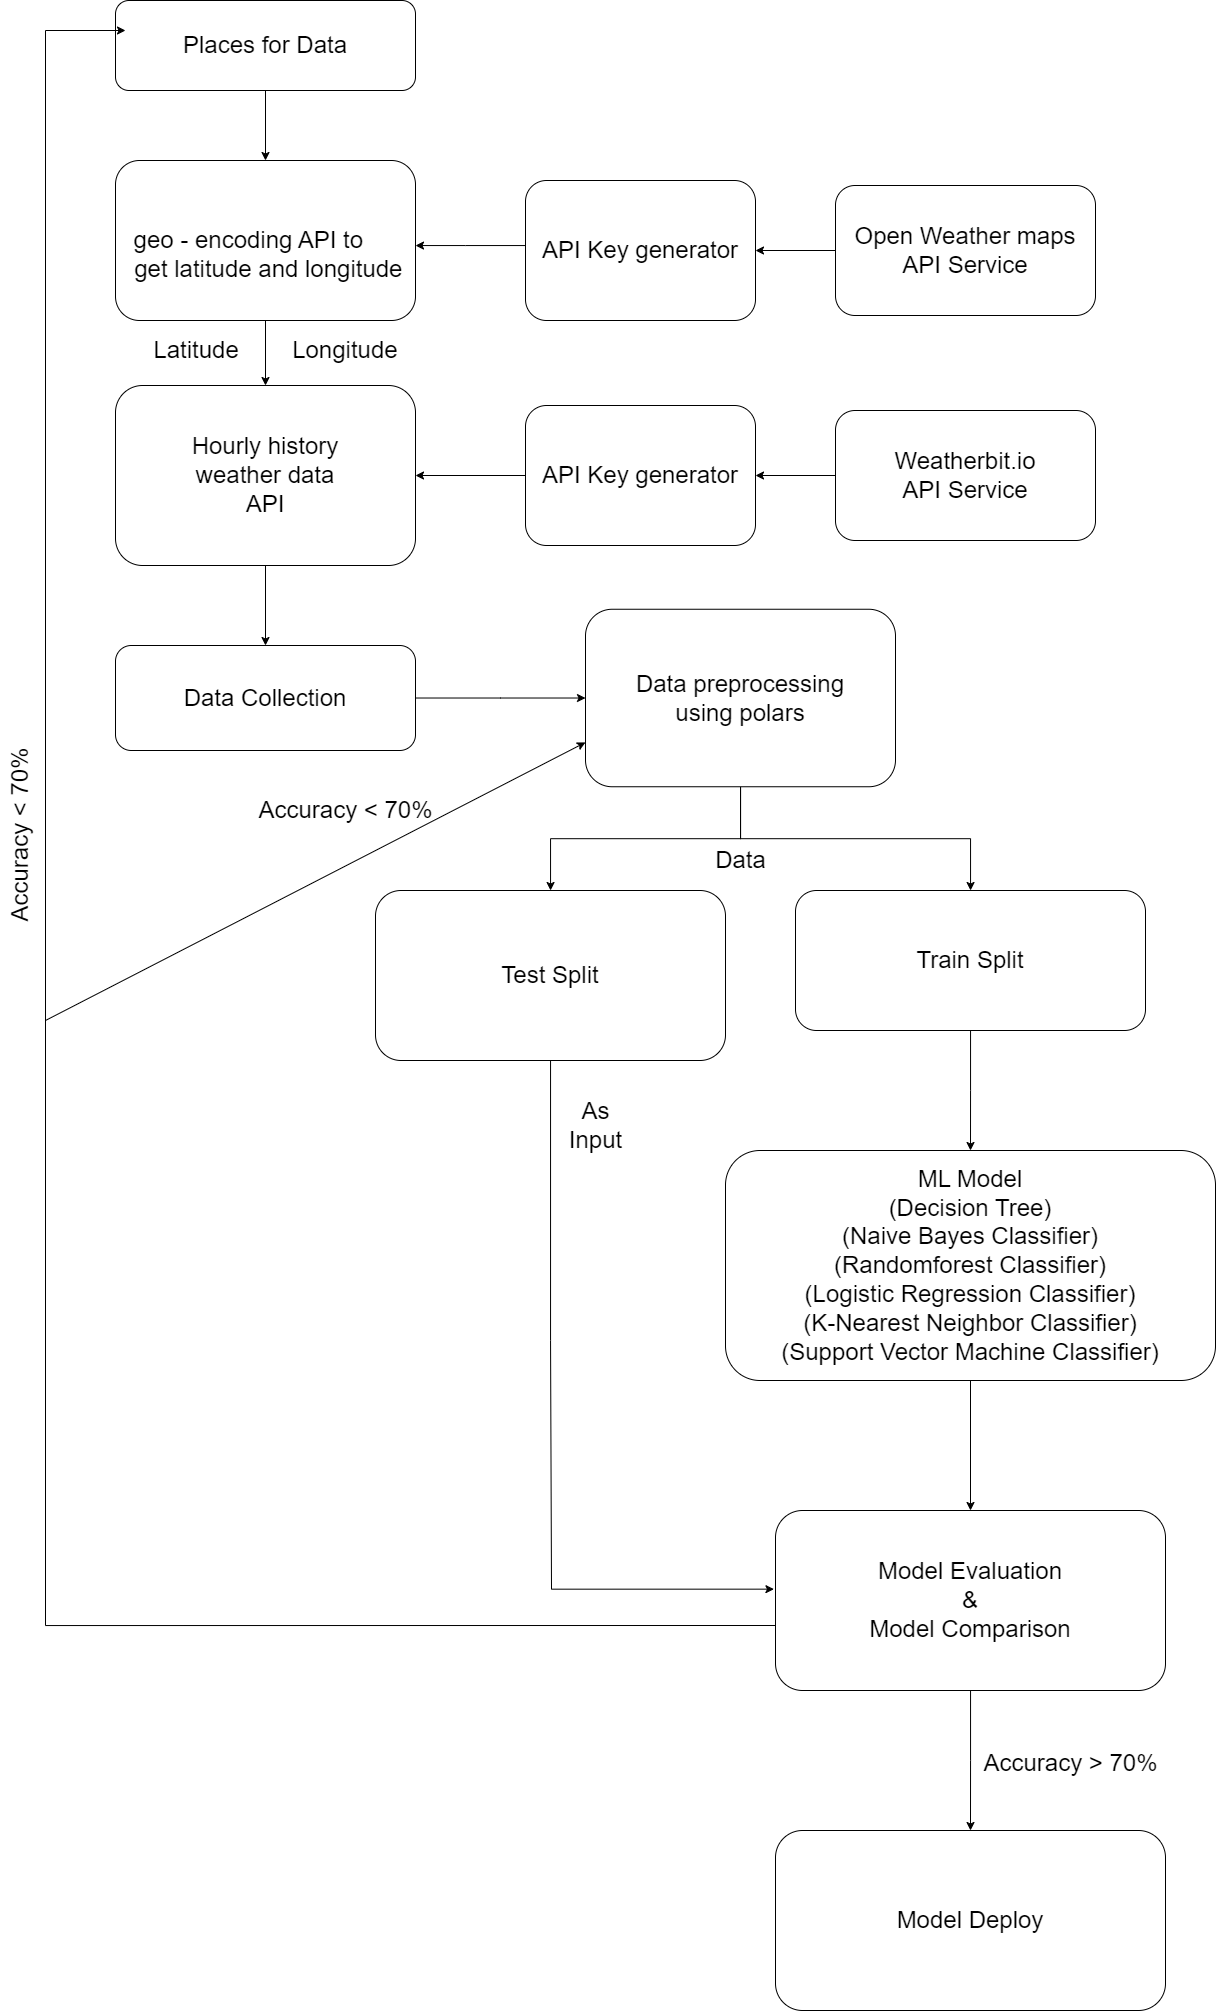
\includegraphics[width=0.81\textwidth]{"../../images/flow_chart.png"} % Replace 'example-image-a' with your image file name
    \caption{Flow Chart}
    \label{Flow Chart}
\end{figure}

\subsection{\textbf{Decision Tree}}
A Decision Tree is a popular and widely used algorithm in machine learning for both classification and regression tasks. It is a versatile and intuitive model that mimics the human decision-making process by breaking down a complex decision into a series of simpler, more manageable decisions. Decision Trees offer a compelling framework for weather prediction due to their inherent ability to handle complex decision-making processes involved in atmospheric conditions. In the context of weather forecasting, a Decision Tree model could effectively evaluate various meteorological factors such as temperature, humidity, wind speed, and atmospheric pressure at different decision nodes. The algorithm's hierarchical structure allows it to capture intricate relationships and interactions among these features, providing a clear and interpretable path to predicting weather outcomes. For instance, the model might start by assessing the temperature range and then branch out to consider humidity levels or wind patterns based on specific thresholds.
\\  \[ H(X) = - \sum_{i=1}^{n} p(x_i) \log_2 p(x_i) \]
\[ IG(T, A) = H(T) - \sum_{v \in \text{Values}(A)} \frac{|T_v|}{|T|} H(T_v) \]
\begin{figure}[htbp]
    \begin{subfigure}{0.33\textwidth}
        \centering
        \includegraphics[width=\linewidth]{"../../images/decision_tree/confusion_matrix_heatmap.png"}
        \caption{Decision Tree Confusion Matrix Heatmap}
        \label{fig:decision_tree_1}
    \end{subfigure}
    \begin{subfigure}{0.33\textwidth}
        \centering
        \includegraphics[width=\linewidth]{"../../images/decision_tree/roc_curve.png"}
        \caption{Decision Tree ROC curve}
        \label{fig:decision_tree_2}
    \end{subfigure}
    \begin{subfigure}{0.33\textwidth}
        \centering
        \includegraphics[width=\linewidth]{"../../images/decision_tree/precision_recall_curve.png"}
        \caption{Decision Tree Precision Recall Curve}
        \label{fig:decision_tree_3}
    \end{subfigure}
    \caption{Decision Tree figures}
    \label{fig:decision_tree}
\end{figure}

\subsection{\textbf{K-Nearest Neighbor Classifier}}
The K-Nearest Neighbor (KNN) classifier, a versatile and intuitive algorithm, finds its application in weather prediction by leveraging the principle of similarity in feature space. In the context of meteorology, KNN operates by identifying the k-nearest historical weather data points to a given input, effectively determining the prevailing weather conditions. The algorithm assumes that similar atmospheric states in the past are indicative of comparable conditions in the future. For instance, if the k-nearest neighbors of a current weather pattern predominantly exhibit rainy conditions, the model predicts rain for the input data point. KNN's adaptability to various types of meteorological data, such as temperature, humidity, and wind speed, makes it well-suited for capturing the intricate relationships within atmospheric variables. However, it's essential to consider the impact of hyperparameter choices, such as the value of k, on the model's performance. Despite its simplicity, the KNN classifier demonstrates effectiveness in weather prediction tasks, particularly in scenarios where the underlying patterns exhibit local coherence and continuity. Moreover, K-Nearest Neighbor (KNN) classifier excels in scenarios where the spatial and temporal aspects of weather patterns play a crucial role. The algorithm does not assume a specific functional form for the underlying relationships but instead relies on the proximity of data points in a high-dimensional feature space. This makes KNN particularly adept at capturing non-linear and complex dependencies that may exist within meteorological data. In the context of weather prediction, where abrupt changes and local variations are common, the ability of KNN to adapt to the local structure of the data becomes advantageous. It becomes a valuable tool in predicting short-term weather conditions and capturing sudden shifts in atmospheric dynamics.
\indent\indent \[ d = \sqrt{(x_2 - x_1)^2 + (y_2 - y_1)^2} \]
\begin{figure}[htbp]
    \begin{subfigure}{0.33\textwidth}
        \centering
        \includegraphics[width=\linewidth]{"../../images/KNeighbors_classifier/confusion_matrix_heatmap.png"}
        \caption{KNeighbors classifier Confusion Matrix Heatmap}
        \label{fig:decision_tree_1}
    \end{subfigure}
    \begin{subfigure}{0.33\textwidth}
        \centering
        \includegraphics[width=\linewidth]{"../../images/KNeighbors_classifier/roc_curve.png"}
        \caption{KNeighbors classifier ROC curve}
        \label{fig:decision_tree_2}
    \end{subfigure}
    \begin{subfigure}{0.33\textwidth}
        \centering
        \includegraphics[width=\linewidth]{"../../images/KNeighbors_classifier/precision_recall_curve.png"}
        \caption{KNeighbors classifier Confusion precision recall curve}
        \label{fig:decision_tree_3}
    \end{subfigure}
    \caption{KNeighbors classifier}
    \label{fig:KNeighbors classifier}
\end{figure}

\subsection{\textbf{Logistic Regression Classifier}}
Logistic Regression, a widely used classification algorithm, finds relevance in weather prediction due to its adaptability to binary outcomes. In the context of weather forecasting, where predicting events like rain or no rain is often pivotal, Logistic Regression proves valuable. Unlike its name might suggest, Logistic Regression is employed for classification tasks, providing the probability of a particular event occurring. In weather prediction, this translates to estimating the likelihood of specific weather conditions based on input features such as temperature, humidity, and wind speed. Logistic Regression models in weather prediction analyze historical data to learn patterns and relationships between these features and the occurrence of weather events. This facilitates the creation of a decision boundary that can distinguish between different weather outcomes. While Logistic Regression may not capture the intricate nuances of complex atmospheric interactions as some advanced models do, its simplicity, interpretability, and efficiency make it a useful tool for certain aspects of weather prediction, particularly in binary weather classification scenarios. When complemented with other sophisticated models, Logistic Regression can contribute to the robustness of a comprehensive weather prediction system.
\\ \[ g(z) = \frac{1}{1 + e^{-z}} \]
\begin{figure}[htbp]
    \begin{subfigure}{0.33\textwidth}
        \centering
        \includegraphics[width=\linewidth]{"../../images/logistic_regression/confusion_matrix_heatmap.png"}
        \caption{Logistic Regression Confusion Matrix Heatmap}
        \label{fig:logistic_regression_1}
    \end{subfigure}
    \begin{subfigure}{0.33\textwidth}
        \centering
        \includegraphics[width=\linewidth]{"../../images/logistic_regression/roc_curve.png"}
        \caption{Logistic Regression ROC curve}
        \label{fig:logistic_regression_2}
    \end{subfigure}
    \begin{subfigure}{0.33\textwidth}
        \centering
        \includegraphics[width=\linewidth]{"../../images/logistic_regression/precision_recall_curve.png"}
        \caption{Logistic Regression Confusion precision recall curve}
        \label{fig:logistic_regression_3}
    \end{subfigure}
    \caption{Logistic Regression}
    \label{fig:Logistic Regression}
\end{figure}

\subsection{\textbf{Naive Bayes Classifier}}
in the realm of weather prediction, the Naive Bayes Classifier emerges as a pragmatic and computationally efficient tool for making predictions based on probabilistic reasoning. This classifier, rooted in Bayes' theorem, assumes independence among features, simplifying the computational complexity while providing surprisingly accurate results. In the context of weather forecasting, where numerous factors contribute to atmospheric conditions, Naive Bayes excels in handling diverse and interrelated features. By leveraging historical weather data, atmospheric pressure readings, wind patterns, and other meteorological parameters, the Naive Bayes Classifier adeptly computes the likelihood of specific weather outcomes. Its ability to swiftly adapt to new data and incorporate real-time information makes it particularly suitable for dynamic weather conditions. Despite its simplicity and the "naive" assumption of feature independence, Naive Bayes has demonstrated notable success in various applications, and its application in weather prediction showcases its versatility in tackling complex datasets. The Naive Bayes Classifier, therefore, stands as a valuable asset in the quest for more accurate and timely weather forecasts.
\\ \[ P(A \mid B) = \frac{P(B \mid A) P(A)}{P(B)} \]
\begin{figure}[htbp]
    \begin{subfigure}{0.33\textwidth}
        \centering
        \includegraphics[width=\linewidth]{"../../images/logistic_regression/confusion_matrix_heatmap.png"}
        \caption{Naive Bayes Confusion Matrix Heatmap}
        \label{fig:naive_bayes_1}
    \end{subfigure}
    \begin{subfigure}{0.33\textwidth}
        \centering
        \includegraphics[width=\linewidth]{"../../images/logistic_regression/roc_curve.png"}
        \caption{Naive Bayes ROC curve}
        \label{fig:navie_bayes_2}
    \end{subfigure}
    \begin{subfigure}{0.33\textwidth}
        \centering
        \includegraphics[width=\linewidth]{"../../images/logistic_regression/precision_recall_curve.png"}
        \caption{Naive Bayes Confusion precision recall curve}
        \label{fig:naive_bayes_3}
    \end{subfigure}
    \caption{Naive Bayes}
    \label{fig:Naive Bayes}
\end{figure}

\subsection{\textbf{Random Forest Classifier}}
Random Forest, a powerful ensemble learning algorithm, holds significant promise in the realm of 	weather prediction. Unlike individual decision trees, 	a Random Forest combines the strength of multiple 	trees to enhance predictive accuracy and robustness. 	In the context of weather forecasting, this approach 	proves invaluable in capturing the intricate and non-	linear relationships within meteorological data. By 	training on diverse subsets of the dataset and 	aggregating predictions, Random Forests excel in 	handling the complexity of atmospheric conditions. 	The algorithm's ability to mitigate overfitting, a 	common challenge in weather prediction models, 	ensures a more reliable and generalizable 	performance. Additionally, Random Forests provide 	a natural mechanism for feature importance 	assessment, aiding meteorologists in identifying the 	key variables driving accurate predictions. The 	adaptability of Random Forests to various 	geographical locations and their capacity to handle 	real-time data make them a compelling choice for 	advancing the precision and reliability of weather 	forecasts. As weather patterns are inherently 	dynamic and multifaceted, the ensemble nature of 	Random Forests positions them as a potent tool for 	addressing the intricacies of meteorological 	prediction and contributing to the ongoing evolution 	of forecasting models.
\\  \[ H(X) = - \sum_{i=1}^{n} p(x_i) \log_2 p(x_i) \]
\[ IG(T, A) = H(T) - \sum_{v \in \text{Values}(A)} \frac{|T_v|}{|T|} H(T_v) \]
\begin{figure}[htbp]
    \begin{subfigure}{0.33\textwidth}
        \centering
        \includegraphics[width=\linewidth]{"../../images/random_forest/confusion_matrix_heatmap.png"}
        \caption{Random Forest Confusion Matrix Heatmap}
        \label{fig:random_forest_1}
    \end{subfigure}
    \begin{subfigure}{0.33\textwidth}
        \centering
        \includegraphics[width=\linewidth]{"../../images/random_forest/roc_curve.png"}
        \caption{Random Forest ROC curve}
        \label{fig:random_forest_2}
    \end{subfigure}
    \begin{subfigure}{0.33\textwidth}
        \centering
        \includegraphics[width=\linewidth]{"../../images/random_forest/precision_recall_curve.png"}
        \caption{Random Forest Confusion precision recall curve}
        \label{fig:random_forest_3}
    \end{subfigure}
    \caption{Random Forest}
    \label{fig:Random Forest}
\end{figure}

\subsection{\textbf{SVM Classifier}}
Support Vector Machines (SVM) classifiers have proven to be effective tools in the domain of weather prediction, offering unique advantages in handling complex and non-linear relationships within meteorological datasets. SVMs excel in scenarios where the underlying patterns are intricate and not easily discernible through linear methods. In the context of weather prediction, SVMs leverage a kernel trick that allows them to implicitly map input features into a higher-dimensional space, making it possible to discern subtle patterns in the atmospheric data. This is particularly beneficial when dealing with variables such as temperature, humidity, and wind patterns, which often exhibit non-linear relationships. SVMs are adept at finding optimal hyperplanes that separate different weather conditions, allowing for accurate classification of distinct meteorological states. Furthermore, their ability to handle high-dimensional data, coupled with the flexibility in choosing different kernel functions, empowers SVMs to capture and understand the intricate interactions among various atmospheric parameters. As weather systems involve multiple contributing factors, the robust nature of SVMs positions them as valuable tools for improving the accuracy and reliability of weather prediction models.
\\ \[ f(X) = w \cdot X + b \]
\begin{figure}[htbp]
    \begin{subfigure}{0.33\textwidth}
        \centering
        \includegraphics[width=\linewidth]{"../../images/svm/confusion_matrix_heatmap.png"}
        \caption{SVM Classifier Confusion Matrix Heatmap}
        \label{fig:SVM_classifier_1}
    \end{subfigure}
    \begin{subfigure}{0.33\textwidth}
        \centering
        \includegraphics[width=\linewidth]{"../../images/svm/roc_curve.png"}
        \caption{SVM Classifier ROC curve}
        \label{fig:SVM_classifier_2}
    \end{subfigure}
    \begin{subfigure}{0.33\textwidth}
        \centering
        \includegraphics[width=\linewidth]{"../../images/svm/precision_recall_curve.png"}
        \caption{SVM Classifier Confusion precision recall curve}
        \label{fig:SVM_classifier_3}
    \end{subfigure}
    \caption{SVM Classifier}
    \label{fig:SVM Classifier}
\end{figure}

\section{Results and analysis}
\begin{table}[ht]
    \centering
    \caption{Performance Metrics for Various Algorithms}
    \label{tab:performance_metrics}
    \resizebox{0.9\textwidth}{!}{
    \renewcommand{\arraystretch}{2.1} % adjust row height
      \fontsize{18}{24}\selectfont
      \begin{tabular}{|l|c|c|c|c|c|}
          \hline
          \textbf{Algorithm} & \textbf{True Positive} & \textbf{True Negative} & \textbf{False Positive} & \textbf{False Negative} & \textbf{Accuracy (\%)} \\
          \hline
          Decision Tree & 509 & 568 & 166 & 93 & 80.61 \\
          \hline
          K-Nearest Neighbor Classifier & 601 & 459 & 74 & 202 & 79.34 \\
          \hline
          Logistic Regression & 475 & 491 & 200 & 170 & 72.30 \\
          \hline
          Naive Bayes & 550 & 465 & 125 & 196 & 75.97 \\
          \hline
          Random Forest & 617 & 575 & 86 & 58 & 89.22 \\
          \hline
          Support Vector Machine & 465 & 509 & 210 & 152 & 72.90 \\
          \hline
      \end{tabular}
    }
\end{table}

\section{\textbf{conclusion}}
After evaluating various machine learning algorithms for rainfall prediction, SVM, logistic regression, and Naive Bayes fell short of the desired 80\% accuracy threshold. K-Nearest Neighbors exhibited promising accuracy but raised concerns about prediction bias. Decision Tree faced challenges with a significant imbalance in true positives and true negatives. In contrast, the Random Forest Classifier emerged as the optimal choice, demonstrating commendable accuracy and a balanced distribution in the confusion matrix, highlighting its effectiveness for the rainfall prediction project.
\\ \indent The evaluation of diverse machine learning algorithms on our dataset reveals valuable insights into their performance, guiding our selection for deployment. SVM, logistic regression, and Naive Bayes exhibited suboptimal accuracy, failing to reach the desired 80\% threshold even after rigorous preprocessing. On the other hand, K-Nearest Neighbors Classifier demonstrated promising accuracy, yet its noticeable disparity between true positive and true negative values raised concerns about prediction bias. Decision Tree also faced challenges, showing a significant imbalance in true positives and true negatives. In contrast, the Random Forest Classifier emerged as the most compelling choice. It not only exhibited commendable accuracy but also maintained a more balanced distribution between true positives and true negatives in the confusion matrix. This dual prowess positions the Random Forest Classifier as the model of choice for our rainfall prediction project. Our findings underscore the significance of algorithm selection and the substantial impact it can have on predictive performance. In the pursuit of deploying an accurate and robust model, the Random Forest Classifier stands out as the optimal solution, showcasing its ability to navigate the intricacies of our dataset effectively. This conclusion is pivotal for the successful implementation of our proposed work, emphasizing the importance of thoughtful algorithm selection in the realm of rainfall prediction.

\begin{thebibliography}{00}
\bibitem{b1} K. P. Selvam and M. Brorsson, "Performance Modeling of Weather Forecast Machine Learning for Efficient HPC," 2022 IEEE 42nd International Conference on Distributed Computing Systems (ICDCS), Bologna, Italy, 2022, pp. 1268-1269, doi: 10.1109/ICDCS54860.2022.00127. keywords: {Training;Analytical models;Computational modeling;High performance computing;Weather forecasting;Predictive models;Benchmark testing;High-Performance Computing;Deep Learning;Weather Forecast;Distributed Computing;Performance modeling;Benchmark Analysis},
\bibitem{b2} M. Pérez-Ortiz, P. A. Gutiérrez, P. Tino, C. Casanova-Mateo and S. Salcedo-Sanz, "A mixture of experts model for predicting persistent weather patterns," 2018 International Joint Conference on Neural Networks (IJCNN), Rio de Janeiro, Brazil, 2018, pp. 1-8, doi: 10.1109/IJCNN.2018.8489179. keywords: {Predictive models;Atmospheric modeling;Airports;Artificial neural networks;Weather forecasting;mixture of experts;persistence model;dynamic systems;ordinal classification;ordinal regression;autoregressive models;neural networks;low-visibility},
\bibitem{b3} M. S. Pathan, A. Nag and S. Dev, "Efficient Rainfall Prediction Using a Dimensionality Reduction Method," IGARSS 2022 - 2022 IEEE International Geoscience and Remote Sensing Symposium, Kuala Lumpur, Malaysia, 2022, pp. 6737-6740, doi: 10.1109/IGARSS46834.2022.9884849. keywords: {Dimensionality reduction;Analytical models;Geoscience and remote sensing;Predictive models;Feature extraction;Task analysis;Meteorology;rainfall prediction;machine learning;dimensionality reduction;feature selection;principal component analysis},
\bibitem{b4} B. Kravets, M. -L. Kloubert, N. Voigt and J. Kays, "Development and Application of a Machine Learning-Based Load Flow Forecast," ETG Congress 2023, Kassel, Germany, 2023, pp. 1-6.
\bibitem{b5} R. Balamurugan, K. Choudhary and S. P. Raja, "Prediction of Flooding Due to Heavy Rainfall in India Using Machine Learning Algorithms: Providing Advanced Warning," in IEEE Systems, Man, and Cybernetics Magazine, vol. 8, no. 4, pp. 26-33, Oct. 2022, doi: 10.1109/MSMC.2022.3183806. keywords: {Support vector machines;Machine learning algorithms;Precipitation;Stacking;Sea measurements;Predictive models;Real-time systems;Floods},
\bibitem{b6} Sue Ellen Haupt, Jim Cowie, Seth Linden, Tyler McCandless, Branko Kosovic, Stefano Alessandrini,†Machine Learning for Applied Weather Prediction, 2018 IEEE 14th International Conference on e-Science.
\bibitem{b7} Ye Ding, Member, IEEE, Yanhua Li, Senior Member, IEEE, Ke Deng, Member, IEEE, Haoyu Tan, Member, IEEE, Mingxuan Yuan, Member, IEEE, Lionel M. Ni, Fellow, IEEE, Detecting and Analyzing Urban Regions with High Impact of Weather Change on Transport.10.1109/TBDATA.2016.2623320,IEEE.
\bibitem{b8} Deepti Gupta, Udayan Ghose,†A Comparative Study of Classification Algorithms for Forecasting Rainfall, 2015 IEEE.
\bibitem{b9} E. B. Abrahamsen, O. M. Brastein, B. Lie, Machine Learning in Python for Weather Forecast based on Freely Available Weather Data,†Proceedings of The 59th Conference on Simulation and Modelling (SIMS 59), 26-28 September 2018, Oslo Metropolitan University, Norway.
\bibitem{b10} Y.Radhika and M.Shashi, Atmospheric Temperature Prediction using Support Vector Machines,†International Journal of Computer Theory and Engineering, Vol. 1, No. 1, April 2009 1793-8201.
\bibitem{b11} Antonio S. Cofıno˜ and Rafael Cano and Carmen Sordo and Jose M. Guti ´ errez ´, Bayesian Networks for Probabilistic Weather Prediction. in ECAI 2002. Proceedings of the 15th European Conference on Artificial Intelligence, IOS Press, 695 - 700 (2002).
\bibitem{b12} Mohsen Hayati, and Zahra Mohebi, Application of Artificial Neural Networks for Temperature Forecasting, World Academy of Science, Engineering and Technology International Journal of Electrical, Computer, Energetic, Electronic and Communication Engineering Vol:1, No:4, 2007.
\bibitem{b13} S Karmakar, M K Kowar, P Guhathakurta,†Long-Range Monsoon Rainfall Pattern Recognition \& Prediction for the Subdivision ˜EPMB™ Chhattisgarh Using Deterministic \& Probabilistic Neural Network, 2009 Seventh International Conference on Advances in Pattern Recognition.
\bibitem{b14} Navin Sharma, Pranshu Sharma, David Irwin, and Prashant Shenoy, Predicting Solar Generation from Weather Forecasts Using Machine Learning, ©2011 IEEE.
\end{thebibliography}
\vspace{12pt}
\color{red}

\end{document}


